% This is "sig-alternate.tex" V1.9 April 2009
% This file should be compiled with V2.4 of "sig-alternate.cls" April 2009
%
% This example file demonstrates the use of the 'sig-alternate.cls'
% V2.4 LaTeX2e document class file. It is for those submitting
% articles to ACM Conference Proceedings WHO DO NOT WISH TO
% STRICTLY ADHERE TO THE SIGS (PUBS-BOARD-ENDORSED) STYLE.
% The 'sig-alternate.cls' file will produce a similar-looking,
% albeit, 'tighter' paper resulting in, invariably, fewer pages.
%
% ----------------------------------------------------------------------------------------------------------------
% This .tex file (and associated .cls V2.4) produces:
%       1) The Permission Statement
%       2) The Conference (location) Info information
%       3) The Copyright Line with ACM data
%       4) NO page numbers
%
% as against the acm_proc_article-sp.cls file which
% DOES NOT produce 1) thru' 3) above.
%
% Using 'sig-alternate.cls' you have control, however, from within
% the source .tex file, over both the CopyrightYear
% (defaulted to 200X) and the ACM Copyright Data
% (defaulted to X-XXXXX-XX-X/XX/XX).
% e.g.
% \CopyrightYear{2007} will cause 2007 to appear in the copyright line.
% \crdata{0-12345-67-8/90/12} will cause 0-12345-67-8/90/12 to appear in the copyright line.
%
% ---------------------------------------------------------------------------------------------------------------
% This .tex source is an example which *does* use
% the .bib file (from which the .bbl file % is produced).
% REMEMBER HOWEVER: After having produced the .bbl file,
% and prior to final submission, you *NEED* to 'insert'
% your .bbl file into your source .tex file so as to provide
% ONE 'self-contained' source file.
%
% ================= IF YOU HAVE QUESTIONS =======================
% Questions regarding the SIGS styles, SIGS policies and
% procedures, Conferences etc. should be sent to
% Adrienne Griscti (griscti@acm.org)
%
% Technical questions _only_ to
% Gerald Murray (murray@hq.acm.org)
% ===============================================================
%
% For tracking purposes - this is V1.9 - April 2009

\documentclass{sig-alternate}

\usepackage{amssymb}
\setcounter{tocdepth}{3}
\usepackage{graphicx}
\usepackage{xcolor}
\usepackage{subfigure} %[tight,normalsize]
\usepackage{algorithmic}
\usepackage{algorithm}
\usepackage{textcomp}
\usepackage{listings}
\usepackage[T1]{fontenc}
\usepackage{hyperref}
\usepackage{cite} %after hyperref

%\usepackage{url}
%\urldef{\mailsa}\path|{alfred.hofmann, ursula.barth, ingrid.haas, frank.holzwarth,|
%\urldef{\mailsb}\path|anna.kramer, leonie.kunz, christine.reiss, nicole.sator,|
%\urldef{\mailsc}\path|erika.siebert-cole, peter.strasser, lncs}@springer.com|    
%\newcommand{\keywords}[1]{\par\addvspace\baselineskip
%\noindent\keywordname\enspace\ignorespaces#1}

\begin{document}


%
% --- Author Metadata here ---
\conferenceinfo{ESEC/FSE}{'11 SZEGED, HUNGARY}
%\CopyrightYear{2007} % Allows default copyright year (20XX) to be over-ridden - IF NEED BE.
%\crdata{0-12345-67-8/90/01}  % Allows default copyright data (0-89791-88-6/97/05) to be over-ridden - IF NEED BE.
% --- End of Author Metadata ---

%\title{Debugging by {\huge\bf\textit{lastChange}}}
\title{\huge\bf{Querypoint} : Moving Backwards on Wrong Values in the Buggy Execution}

%\subtitle{[Extended Abstract]
%\titlenote{A full version of this paper is available as
%\textit{Author's Guide to Preparing ACM SIG Proceedings Using
%\LaTeX$2_\epsilon$\ and BibTeX} at
%\texttt{www.acm.org/eaddress.htm}}}

%
% You need the command \numberofauthors to handle the 'placement
% and alignment' of the authors beneath the title.
%
% For aesthetic reasons, we recommend 'three authors at a time'
% i.e. three 'name/affiliation blocks' be placed beneath the title.
%
% NOTE: You are NOT restricted in how many 'rows' of
% "name/affiliations" may appear. We just ask that you restrict
% the number of 'columns' to three.
%
% Because of the available 'opening page real-estate'
% we ask you to refrain from putting more than six authors
% (two rows with three columns) beneath the article title.
% More than six makes the first-page appear very cluttered indeed.
%
% Use the \alignauthor commands to handle the names
% and affiliations for an 'aesthetic maximum' of six authors.
% Add names, affiliations, addresses for
% the seventh etc. author(s) as the argument for the
% \additionalauthors command.
% These 'additional authors' will be output/set for you
% without further effort on your part as the last section in
% the body of your article BEFORE References or any Appendices.

\numberofauthors{3} %  in this sample file, there are a *total*
% of EIGHT authors. SIX appear on the 'first-page' (for formatting
% reasons) and the remaining two appear in the \additionalauthors section.
%
\author{
% You can go ahead and credit any number of authors here,
% e.g. one 'row of three' or two rows (consisting of one row of three
% and a second row of one, two or three).
%
% The command \alignauthor (no curly braces needed) should
% precede each author name, affiliation/snail-mail address and
% e-mail address. Additionally, tag each line of
% affiliation/address with \affaddr, and tag the
% e-mail address with \email.
%
% 1st. author
\alignauthor
Salman Mirghasemi\\
       \affaddr{\'Ecole Polytechnique F\'ed\'erale de Lausanne (EPFL), Switzerland}\\
       \email{salman.mirghasemi@epfl.ch}
% 2nd. author
\alignauthor
John J. Barton\\
       \affaddr{IBM Research - Almaden}\\
       \email{bartonjj@us.ibm.com}
% 3rd. author
\alignauthor 
Claude Petitpierre\\
       \affaddr{\'Ecole Polytechnique F\'ed\'erale de Lausanne (EPFL), Switzerland}\\
       \email{claude.petitpierre@epfl.ch}
}       

% There's nothing stopping you putting the seventh, eighth, etc.
% author on the opening page (as the 'third row') but we ask,
% for aesthetic reasons that you place these 'additional authors'
% in the \additional authors block, viz.
% Just remember to make sure that the TOTAL number of authors
% is the number that will appear on the first page PLUS the
% number that will appear in the \additionalauthors section.

\maketitle

\begin{abstract}

\end{abstract}
Developers often seek the origins of wrong values they see in their
debugger. Their search must be backwards in time: the code causing the
wrong value executed before the wrong value appeared. Searching with
breakpoint- or log- based debuggers demands persistence and significant experience with the application being debugged.  

\textit{Querypoint}, is a Firefox plugin which enhances the popular Firebug JavaScript debugger with
 a new, practical feature called \textit{lastChange}, which automatically locates the last point that a variable 
or an object property has been changed. Starting from a program halted on a breakpoint, the \textit{lastChange} solution
applies queries to the live program during re-execution, recording the call stack and limited program state each time 
the property value changes. When the program halts again on the breakpoint, the recorded information can be shown to the developer.


\category{D.2.5}{Testing and Debugging}{Debugging aids}
\category{D.2.6}{Programming Environments}{Integrated environments}


\terms
{Algorithms, Human Factors, Languages}

\keywords
{Debugging, Locating Defects, Querypoint, LastChange, Breakpoint,
 Watchpoint, Logging}

\section{Introduction}

According to  \cite{LaToza}, developers spend about fifty percent of
their time debugging. To fix a bug, developers typically reproduce 
and monitor the buggy execution several times to understand the 
program's unexpected behavior. Trial-and-error, guess-work, and 
analyzing complicated data make debugging difficult and time-consuming. 
Enhanced debugging operations save  
time, reduce development costs and improve software quality.

A common strategy for locating defects starts from bug symptoms and
works backwards, moving from a point in the program execution where a
value appears to be incorrect back to the point where that value was
set.  Two conventional approaches, breakpoint-based and
log-based debugging, require tedious steps of
selecting data to be collected, collecting the data, then analyzing
the results. 

In breakpoint debugging, developers select data to be collected by
searching through source files and setting breakpoints. To determine
where a value was set incorrectly, a developer must set
breakpoints at all possible points where the value changes. At
every breakpoint, the developer must determine if the location is in
fact related to the questionable value change then study the complex
debugger user interface and memorize values or manually collect
data. As the number of breakpoint hits increases, the process of
checking the program state, collecting data and resuming the execution
becomes cumbersome.

In log-based debugging, developers select data to be collected by
inserting statements for all points of possible change.  While in
breakpoint-based debugging, the whole program state is available to
developer, in log-based debugging, developer has to decide what data
should be collected when inserts the log statement. It is very common
that the developer has to repeat this step several times due to
insufficient collected data, or to wait a long time because too much
data is recorded. Once adequate data is collected, it still
requires analyzing and understanding. Developers usually end up in
dealing with long log files and analyzing huge amounts of collected data. 
Neither approach effectively assists the developer in finding origins to a wrong
value.

Our new functionality in
debuggers, \textit{lastChange}, locates the origin of a wrong
value by queries on the running program.
Imagine that a program execution is
paused on a breakpoint and the developer is
suspicious about the value of a variable or an object property. The
developer selects \textit{lastChange} on the value. The debugger
replays the buggy execution and collects data
when the data field changes. Once the execution reaches the same place 
(i.e., the same
breakpoint hit), it pauses the execution, analyzes the collected data
and shows the location of the last change to the developer. The
developer can also examine the program state at the located point of
execution, and continue debugging by more \textit{lastChange} queries
from that point.

Our contribution in this paper is the technique \textit{lastChange},
which locates the last place a value has changed, gathers other values
from that execution point, and allows \textit{lastChange} operations
from that point. The technique builds on existing breakpoint debugger
technology  and it does not require a special environment to
create identical, instruction by instruction, re-executions. We demonstrate the feasibility of the approach with 
\textit{Querypoint}, an implementation extending Firebug
JavaScript debugger. \textit{Querypoint} also provides mechanism for
automated bug reproduction, and a novel user interface which
summarizes investigated execution points and collected results.
The \textit{lastChange} algorithm provides information on important program
values during the program execution without voluminous logs and without tedious
 insertion and removal of breakpoints. We believe other queries over the
 running program can be formulated to generalize this technique.

\section{Related Work}
\label{sec:relatedWork}
%whyline, firecrystal

Tools developed to enhance developers' movement on the buggy execution can be classifed in two groups: replay-based and logging-based.

%The algorithm we presented in this paper obtain information about
%the execution state logically earlier in the control flow by querying 
%the executioin state during replay using the technology of 
%conventional breakpoint debuggers.  
The \textit{lastChange} approach resembles the operational model of replay-based debugging 
and the query approach of logging-based
debugging.  Replay-based approaches capture limited data during
execution and replay the buggy execution to reach past points. In
contrast, logging-based approaches collect enough data during
execution to relieve developer from re-execution, then query the data to 
inform the developer. Replay-based
approaches impose much less runtime overhead (about two orders of
magnitudes) comparing to logging-based approaches. However, developer
has to re-execute the buggy execution several
times. \textit{lastChange} collects data on re-execution by queries
selected by developer interaction with the debugger. Therefore it has 
the selectivity of the replay-based approaches that improves performance, 
% but we have 
and the flexibilty of the queries so it does not require deterministic replay.

Among replay-based debuggers we compare to bdb \cite{Boothe} and
reverse watchpoint \cite{Maruyama}.  A bidirectional C debugger, bdb
employs a step counter to locate the requested point from the
beginning of execution. It relies on deterministic execution replay
%(i.e., the same sequence of instructions in re-execution) 
and records the results of non-deterministic system calls and re-injects them into
the program when it is replayed. It makes use of checkpoints to reduce
the time needed for re-execution. Reverse watchpoint, similar to bdb, uses
a counter to correctly locate the last write access of a selected variable in the
next execution \cite{Maruyama}.
% Reverse watchpoint is proposed by Maruyama et al., analyses the execution and moves the debugger to the
% last write access of a selected variable by re-executing the program
%from the beginning\cite{Maruyama}.  Similar to bdb it relies on deterministic
%replay and uses a counter to correctly locate a point in the next
%execution. 
The main disadvantage of these approaches is that they require 
identical, instruction by instruction, re-executions. % exactly the same executions. 
Even one instruction difference between
two executions leads to wrong results. On the other hand,
\textit{lastChange} doesn't require any special feature in the
re-execution and fits into existing debugging practice

Among logging-based approaches are \textit{omniscient} debuggers
ODB\cite{Lewis} and Unstuck\cite{Hofer}. Both
approaches keep the log history in memory and hence can only record
and store the complete history for a short period of time. These
debuggers record all the events that occur during the buggy execution
and later let the developer to navigate through the obtained execution
log. In these approaches there is no execution to resume: moving
backwards in the log can be similar to moving forwards. A more scalable 
approach to omniscient debugging has been proposed by Pothier et al. \cite{Pothier}. 
Their back-in-time debugger, TOD, addresses the space problem by storing 
execution events in a distributed database. Bhansali et al. \cite{Bhansali} attempted to address the performance overhead 
and large trace size of logging-based debugging in their time-travelling debugger, Nirvana. 
Nirvana first collects a full compressed trace of program execution and then 
simulates re-execution. Their results are quite similar to omniscient 
debuggers. Nirvana incurs about 15 to 68 times runtime overhead in 
re-simulation.


Logging-based debuggers suffer from different issues. First, the recording
step is time expensive and it should be repeated in case of changes in
program. Second, the execution log cannot fully replace the live
execution. There are other aspects of execution (e.g., program user
interface, file system, database tables, etc.) which are also
important in debugging and are not available to the developer in 
logging-based debuggers. Third, querying collected data (e.g., to restore
the program state at a certain point) may not be efficient enough for
debugging realistic programs. Comparing to logging-based debuggers our approach 
has little upfront cost and more flexibility. The developer can start debugging just 
after reproducing the bug without a capturing step.  Changing inputs or
environment settings and re-executing to investigate the bug works as
in conventional breakpoint debuggers.


A recent work by Lienhard et al.\cite{Lienhard} suggests virtual
machine level support for keeping the history of events. It replaces every
object reference with an alias object which keeps the history of
changes to the object reference. 
%In this way, when an object is
%collected by garbage collector, its track of changes (if it is not
%referenced by other aliases) will be also collected. 
Although this approach incurs less runtime overhead (7 times) in
comparison to omniscient debuggers, it adds memory
overhead. 

Origin tracking of \texttt{undefined} and \texttt{null} values employing \textit{value piggybacking} technique proposed by
Bond et al. \cite{Bond}. This approach has two main limitations comparing to \textit{lastChange}.
First, it is limited to \texttt{undefined} and \texttt{null} values. Second, it does not return the last change
of a \texttt{null} variable but the first place that the \texttt{null} value is originated.


%Two new directions in logging debuggers explore more detailed use of
%the log and more effective user interface to the collected data. %logging approaches. 
%WhyLine\cite{Ko} provides visual interface to collected runtime information and lets
%developer moves on execution log using queries expressed in terms of
%the programming objects. 

WhyLine\cite{Ko} stores the program user interface in
addition to the program trace and provides answers to why and why not
questions to the user. 
%Jive\cite{Czyz} depicts the history of
%execution by a sequence diagram and lets the user to query on the events
%database. 
WhyLine suffers from the requirement of gathering tracing information before its unique capabilities can be used.
We imagine that the runtime queries we use in \textit{lastChange} may be used to gather data incrementally for this kind of debugging approach.

%Querypoint debugging uses re-executions to gather infor-mation requested by the developer: the memory overhead depends on the query not the entire program. Moreover, the Lienhard et al. debugger significantly changes the virtual machine, while our approach is a generalization to conditional breakpoints and available debugger infrastructure can be adapted to support it.
 
%\textit{lastChange} functionality does rely on a conventional breakpoint to begin queries, a requirement not shared by full logging solutions.  Here we leverage past experience of developers, but there are also new tools [] to help with this problem in the case of graphical and event based systems.



\section{Introductory example}
\label{sec:introExample}

We illustrate the \textit{lastChange} functionality by a simple
example. The example demonstrates a buggy JavaScript code in a HTML
page (Figure~\ref{fig:js-code}). The page contains a button (line 40)
showing the value of \texttt{myObject.myProperty}.  When the user
clicks on the button, the \texttt{onClick} function (line 13) is
called. This function increases the value of
\texttt{myObject.myProperty} by one (line 15) and calls
\texttt{updateButton} function which updates the button's text to the new
value (line 22).  Once the page is loaded for the first time the
button shows \texttt{1} as the initial value of
\texttt{myObject.myProperty}.  In practice when the user clicks on the
button, \texttt{0} appears instead of \texttt{2}: there is a bug.


Two other functions are called in \texttt{onClick()}, \texttt{foo()}
and \texttt{bar()}. As developers we often encounter function calls
which seem peripheral to our current concern; they may have been added
by another developer, or we may have forgotten their exact properties
or those properties may have changed, and so on. The difference
between what we expect these functions to do, e.g. nothing
interesting, and what they do in practice may cause bugs.


\begin{figure}[htp]

%\includegraphics[width=.5\textwidth]{
%\begin{verbatim}
\lstset{basicstyle=\scriptsize}
\lstset{emph={myProperty},emphstyle=\textit}
%\lstset{backgroundcolor=\color{yellow}}
\lstdefinelanguage{myLang}
{morekeywords={html, script, button, if, function, var}}

\begin{lstlisting}[frame=single, language=myLang] %, framerule=0pt]

1 <html>
...
5   <script type="text/javascript">
6    myObject = {myProperty : 1};
7    myCondition = {value : 1};
...
13   function onClick(){
14     foo();
15     myObject.myProperty++;
16     bar();
17     ...
18     updateButton();
19   }
20   function updateButton(){
21     var myParagraph =
          document.getElementById("myButton");
22     myButton.innerHTML = myObject.myProperty;
23   }   
24   function foo(){
25  	 myCondition.value = oldValue;
26   }  
27   function bar(){ 
28     if (!myCondition.value)
29         myObject.myProperty = 0;
30   }
31  </script> 
...
40  <button id="myButton" onclick="onClick()">
41  	1 
42  </button>
43 </html>
\end{lstlisting}
%\end{verbatim}
\caption{A Web page containing JavaScript code. Some lines not related to our paper have been elided.}
\label{fig:js-code}
\end{figure}

By browsing through the code or other means\cite{Barton},
 the developer determines that the value displayed on the 
button is set at line 22. Since the displayed value is incorrect we know 
the bug occurred before we hit this line.
To start debugging, the developer sets a breakpoint
on line 22. Once the button is clicked, the execution is paused at line
22. Figure~\ref{fig:example1} shows the Firebug debugger while the
execution is paused. Firebug has several panels (e.g., HTML, CSS,
Script, DOM, etc.) that each demonstrate one aspect of the Web page.
The Script panel contains the list of all loaded source
files and regular debugging facilities such as setting breakpoints and
stepping. To the right of the script panel, the Watch panel shows the program state
where the developer can examine object and variable values. In our case, the
\texttt{myObject.myProperty} value at the paused point is \texttt{0}. We expected this value to be \texttt{2}.


To apply backward search strategy for locating defects, the developer
first needs to know the origin of the wrong value. To achieve this
goal using breakpoints, the developer should search code to find all possible places that
\texttt{myObject. myProperty} might get a new value and set breakpoint at these locations. However, an
object and property can be accessed and changed through different
names and methods. There is no simple way to identify these aliases or
even their total number.  The developer can make a good guess and set
breakpoints on lines where the property seems to be changed. Then they
re-execute the program and examine the state looking for values that
may lead to the incorrect value observed at line 22. All this work
must be repeated if a new alias is discovered or if some
information related to the buggy result was missed while stopped on
one of the breakpoints.

In contrast, we have added a high-level function in the debugger,
\textit{lastChange}, which provides the answer without tedious manual
effort from the developer. By right clicking on
\texttt{myObject.myProperty} in the Watch panel, the developer can run
\textit{lastChange} command (Figure~\ref{fig:example1}). The debugger
re-executes the program and halts again at the breakpoint on line 22.
However, it shows a new panel, called QP, centered on the source at line 29
(Figure~\ref{fig:example3}), the point of \textit{lastChange}.  To
the right, the TraceData panel shows values of properties of the
program state when it passed through line 29.  These two panels
resemble the Script and Watch panels, but they show data collected by
the debugger at one execution point which is now past: these are
\textit{traces} or \textit{logs} of information collected during the re-execution.


\begin{figure*}[htp]

\subfigure[A screen shot of the Firebug debugger while running the example code from Fig.~\ref{fig:js-code}. The Script
  panel is selected; it gives access to
  all loaded source files and allows breakpoints to be set on lines. In this
  figure, the execution is paused at line 22 by a regular
  breakpoint. The Watch panel on the right shows the program state at
  the paused
  point. Developer can query \textit{lastChange} on \texttt{myObject.myProperty} by right-clicking on the value of \texttt{myProperty}. ]{\label{fig:example1}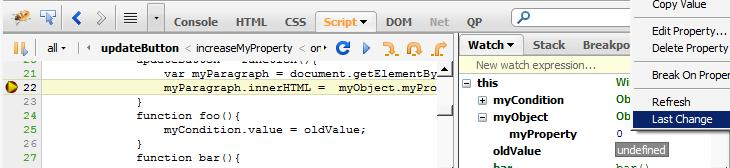
\includegraphics[width=1.0\textwidth, %height=.17\textheight
  ]{1-bp22.jpg}}


\subfigure[The result of \textit{lastChange} query for
  \texttt{myObject.myProperty}. The left panel, QP, shows the source
  code at the point of \textit{lastChange}; The right panel,
  TraceData, shows the collected data at the
  point.]{\label{fig:example3}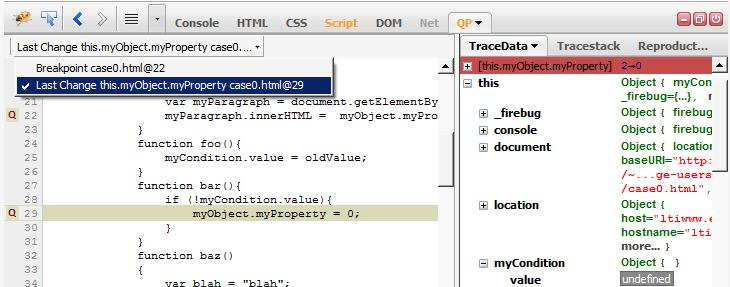
\includegraphics[width=1.0\textwidth,% height=.21\textheight
  ]{3-lastChange.jpg}}

\subfigure[The result of \textit{lastChange} query for
  \texttt{myCondition.value}. To evaluate an expression (e.g., oldValue) at this point, developer can %TODO should we remove it?
  enter the expression in the watch box and after re-execution the result is available.
  The opened list on the top of the left panel shows the visited execution points. Clicking on each point in
  the list shows the corresponding code and
  data.]{\label{fig:example4}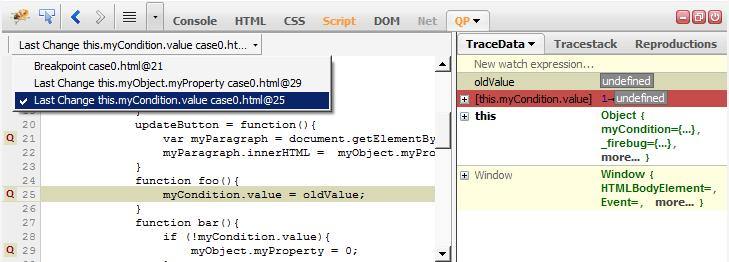
\includegraphics[width=1.0\textwidth%,height=.25\textheight
    ]{4-lastChange2.jpg}}

\caption{The stages of locating the defect using \textit{lastChange} feature.}
\label{fig:lastChange}
\end{figure*}


Looking at line 29, it seems that something is wrong with
\texttt{myCondition.value} which causes line 29 execution. The
developer examines \texttt{myCondition.value} and it is
\texttt{undefined}. The next step is to know when this property got
this value. To do so, the developer runs the \textit{lastChange} command
on \texttt{myCondition.value} at this point. The debugger re-executes the
program and breaks again on line 22, analyzes its queries and shows the developer line 25-the
place \texttt{oldValue} is assigned to
\texttt{myCondition.value}. If the developer asks for \textit{lastChange} on \texttt{oldValue}, 
the debugger can notify the developer that this variable is never assigned a value.
 Now it is clear that the bug occurs because \texttt{oldValue} is
\texttt{undefined} once the execution reaches line 25 (Figure~\ref{fig:example4}).


As demonstrated in Figure~\ref{fig:example-points}, the developer has
examined three points of execution. The first point  was the breakpoint set by the developer. 
We call this special breakpoint the \textit{reproduction point}.
The second and third points preceded the reproduction point in execution sequence.
All three points-the history
of the search for the defect-are available through the debugger's
interface. On the top of the left panel in Figure~\ref{fig:example4}
there is an opened list which shows all three examined points. The
first one is the breakpoint on line 22, the second one is the point
which is when \texttt{myObject.myProperty} changed before
reaching the breakpoint and finally the last one is the point of
execution in which \texttt{myCondition.value} gets the
\texttt{undefined} value. Moreover, the source lines related to these
points are marked with red \textbf{Q} icons.

Notice that in our example, \textit{lastChange} combines some aspects
of breakpoint and of log-based debugging. Like breakpoint debugging,
the developer re-executes a live runtime without changing the source
and without a special execution environment beyond the debugger. The
state of the program memory and the call stack are available at each
lastChange point. Like log-based debugging, the program state and the
call stack are recorded during program execution. We can't halt the
program at \textit{lastChange} because we don't know which point is the last
one until we return to the original breakpoint. In section 5 we
discuss cases where it is possible to pause at lines of \textit{lastChange}.

\subsection{Re-Execution, Reproduction Point and Data Collection}

\section{Limitations and Future Work}

\section{Reproducible Non-Deterministic Execution}

\subsection{Combination of {\large\bf\textit{lastChange}} and Breakpoint Debugging}


\section{Conclusion}

\section{Acknowledgments}

%
% The following two commands are all you need in the
% initial runs of your .tex file to
% produce the bibliography for the citations in your paper.
\bibliographystyle{abbrv}
%\bibliography{sigproc}  % sigproc.bib is the name of the Bibliography in this case
\begin{thebibliography}{16}

\bibitem{Barton}
J.J. Barton, and J. Odvarko. \newblock Dynamic and graphical web page breakpoints.
\newblock In \emph{Conference on World Wide Web(WWW)},
April, 2010.

\bibitem{Bhansali}
S. Bhansali, W. Chen, S. de Jong, A. Edwards, R. Murray, M. Drini\'{c}, D. Miho\v{c}ka, J. Chau. \newblock Framework for instruction-level tracing and analysis of program executions.
\newblock In \emph{International Conference on Virtual Execution Environments(VEE)},
June, 2006.

\bibitem{Bond}%[Bond(2007)]
M.D. Bond, N. Nethercote, S.W. Kent, S.Z. Guyer, and K.S. McKinley. \newblock Tracking bad apples: reporting the origin of null and undefined value errors.
\newblock In \emph{22nd annual ACM SIGPLAN conference on Object-oriented programming, systems, languages, and applications(OOPSLA)},
October, 2007.

%\bibitem{Bond2}%[Bond(2010)]
%M.D. Bond, G.Z. Baker, S.Z. Guyer, and Z. Samuel. \newblock Breadcrumbs: efficient context sensitivity for dynamic bug detection analyses.
%\newblock In \emph{Conference on Programming Language Design and Implementation(PLDI)},
%June, 2010.

\bibitem{Boothe}%[Boothe(2000)]
B. Boothe. \newblock Efficient algorithms for bidirectional debugging.
\newblock In \emph{Conference on Programming Language Design and Implementation(PLDI)},
June, 2000.

%\bibitem{Czyz}%[Czyz(2007)]
%J.K. Czyz, and B. Jayaraman. \newblock Declarative and visual debugging in Eclipse.
%\newblock In \emph{OOPSLA workshop on eclipse technology eXchange},
%October, 2007.

%\bibitem{Firebug}%[Firebug(2010)]
%Firebug. \newblock http://getfirebug.com.

%\bibitem{Firefox}%[Firefox(2010)]
%Firefox. \newblock http://www.mozilla.com.

\bibitem{Hofer}%[Hofer(2006)]
C. Hofer, M. Denker, and S. Ducasse. \newblock Implementing a backward-in-time debugger.
\newblock In Proceedings of\emph{NODe'06},
volume P-88, pages 17-32. Lecture Notes in Informatics, 2006.

\bibitem{Horwitz}%[Hofer(2006)]
S. Horwitz, B. Liblit, and M. Polishchuk. \newblock Better Debugging via Output Tracing and Callstack-Sensitive Slicing.
\emph{IEEE Transactions on
Software Engineering}, 36(1):7-19, 2010.

\bibitem{JPDA}%[JSD(2010)]
Java Platform Debugger Architecture. \newblock http://java.sun.com/javase/technologies/ core/toolsapis/jpda.

\bibitem{Ko}%[Ko(2008)]
A.J. Ko, and B.A. Myers. \newblock Debugging reinvented: asking and answering why and why not questions about program behavior.
\newblock In \emph{30th international conference on Software engineering(ICSE)},
May, 2008.

\bibitem{Korel}%[Ko(2008)]
B. Korel and J. Laski. \newblock Dynamic Program Slicing.
\newblock \emph{Information Processing Letters},
 29(3):155-163, 1988.

\bibitem{LaToza}%[LaToza(2006)]
T.D. LaToza, G. Venolia, and R. DeLine. \newblock Maintaining mental models: a study of developer work habits
\newblock In \emph{28th international conference on Software engineering(ICSE)},
May, 2006.

\bibitem{Lewis}%[Lewis(2003)]
B. Lewis, and M. Ducasse. \newblock Using events to debug Java programs backwards in time.
\newblock In \emph{Companion of the 18th annual ACM SIGPLAN conference on Object-oriented programming, systems, languages, and applications(OOPSLA)},
2003.

\bibitem{Lienhard}%[Lienhard(2008)]
A. Lienhard, T. G\^{\i}rba, and O. Nierstrasz. \newblock Practical Object-Oriented Back-in-Time Debugging.
\newblock In \emph{22nd European conference on Object-Oriented Programming(ECOOP)},
July, 2008.

\bibitem{Maruyama}%[Maruyama(2003)]
K. Maruyama, and T. Kazutaka. \newblock Debugging with Reverse Watchpoint.
\newblock In \emph{Proceedings of the Third International Conference on Quality Software},
2003.

\bibitem{JSD}%[JSD(2010)]
Mozila JavaScript Debugging Interface. \newblock http://www.mozilla.org/js/jsd.

\bibitem{Pothier}%[Pothier(2007)]
G. Pothier, \'{E}. Tanter, and J. Piquer. \newblock Scalable omniscient debugging.
\newblock In \emph{22nd annual ACM SIGPLAN conference on Object-oriented programming, systems, languages, and applications(OOPSLA)},
October, 2007.

\bibitem{Sridharan}%[Boothe(2000)]
M. Sridharan, S.J. Fink , and R. Bodik. \newblock Thin slicing.
\newblock In \emph{Conference on Programming Language Design and Implementation(PLDI)},
June, 2007.

\bibitem{Weiser}
M. Weiser. \newblock Program slicing.
\newblock \emph{IEEE Transactions on
Software Engineering}, vol. SE-10, no. 4, pp. 352-357,
July 1984.

\bibitem{Zeller}
A. Zeller. \newblock Why programs fail: A guide to systematic debugging.
Morgan Kaufmann (2005)

\end{thebibliography}


% You must have a proper ".bib" file
%  and remember to run:
% latex bibtex latex latex
% to resolve all references
%
% ACM needs 'a single self-contained file'!
%
\end{document}
